\section{Постановка задачи}
    Есть некотарая трасса состоящая из двух наборов точек соединенных отрезками,при этом контуры замкнутые ивыпуклая(см рисунок). 

	
	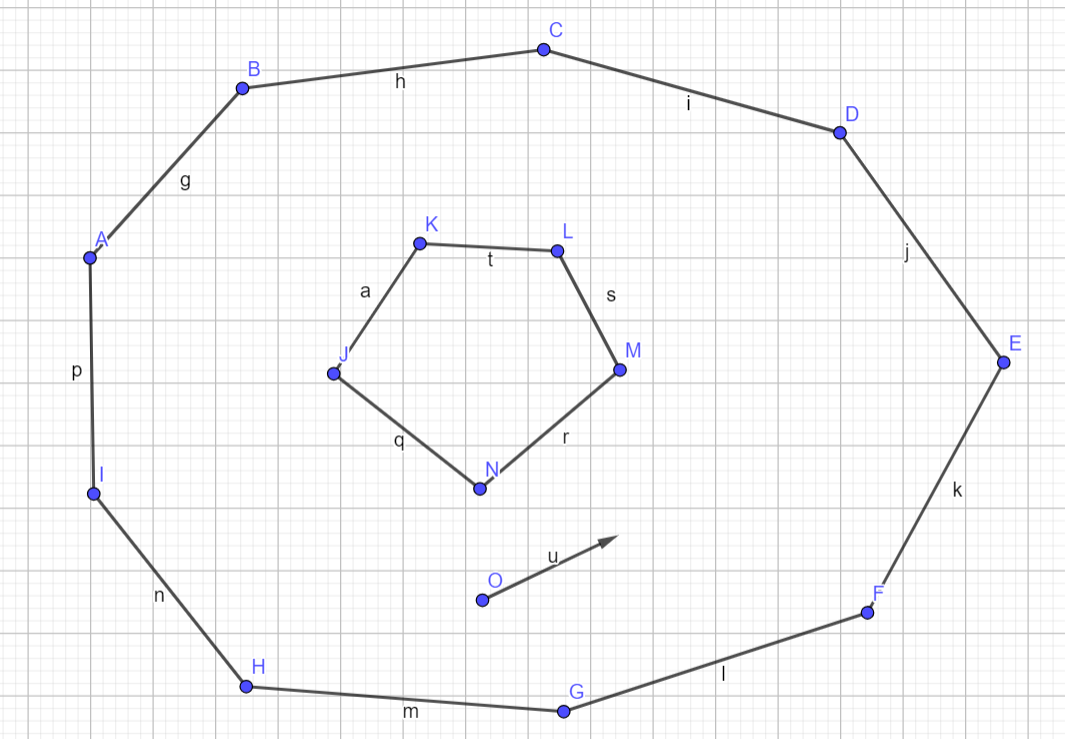
\includegraphics[width=400px]{picture3.png}
	\parskip=0.3cm
	
	Есть точка которая двигается по этой трассе с некоторой постоянной скоростью,которая может менять направления движения через равные промежутки времени.Перед тем как выбрать направление становится известно рассотяние до "стенок" в нескольких направлениях.Необходимо написать программу позволяющую проходить по трассе без "сталкновений" с отрезками как можно дольше.При этом желательно чтобы путь проходил как можно ближе к меньшему контору.
	